%% INTRODUCTION:
%  a. Motivation

The understanding of physical scenes by machines has been of great interest to researchers over the last couple of decades. Being able to construct the three dimensional shape and location of objects in a scene can be very helpful in this task. Based on the observation that, for humans, visual clues seem useful for understanding the structure of their environment, it is not surprising that researchers in the field of computer vision have put great effort in creating methods that reconstruct 3D models out of images. Being able to reconstruct geometry allows for new applications. On a practical level, for example, it allows for easy creation of 3D models for usage in modelling design, computer games and even 3D printing. In addition, geometry reconstruction as an intermediate step opens the door to further processing in advanced street scene understanding, advanced geometry-aware rendering of new content or editing of existing footage (such as changing lighting or virtually moving objects in the scene), navigational tasks in robotic systems, and augmented reality applications\footnote{One could even state that geometry reconstruction could be seen as an intermediate feature in advanced computer vision, much in the same way as edge detection is used extensively as a feature in more advanced image processing algorithms.}. Increasing computer power, cheap and ubiquitous cameras, and recent developments in the field of computer vision and machine learning all help making these exciting applications a reality.

%  b. Problem statement
There has been published a great amount of research on geometry reconstruction. A variety of approaches has been proposed, each with their own advantages and disadvantages. Most, if not all, of the approaches seem to be based on one or more visual clues that are relatively easy to find automatically, such as silhouettes, corner points or similarly coloured pixels in images. Different visual clues call for various requirements in the input images, resulting in successes and failures specific for the chosen approach. Current approaches often rely on the ability to detect features such as silhouettes or distinctive corner points on \emph{all} geometry, resulting in bad results for objects where the specific features are less present.

However, detected features are not the only piece of information that can be used for geometry reconstruction; failure of detection can provide useful information too. Detection failures can be detected by using information from features detected in other parts of the data (\eg other images). In particular, the absence of features in images where they would have been expected - due to detection in images taken from surrounding camera poses - may indicate the existence of other objects. Although this observation might seem obvious, it has not got a lot of attention in the computer vision literature. Bad matches or the absence of features have mostly been treated as outliers or as a binary vote for not using certain data in a particular step in the reconstruction; seldomly has it been used actively for reconstructing geometry\footnote{It is almost as if researchers are afraid of negative information.}. Often camera poses are thrown away after triangulating the feature locations, continuing with the positive information (features) only. Intuitively, this seems like throwing away useful information. It is this intuition that motivates the approach taken in this thesis.

In this thesis, a framework is proposed that uses both \emph{visibility} (detected features) and \emph{occlusion} (undetected but expected features) in order to find, and reconstruct, objects not rich in reliable features. The proposed method uses features detected in other parts of the scene to find objects difficult to detect directly. Based on the visibility and occlusion information of features from given observation locations, space is `carved' in a probabilistic way. The method has been tested on a variety of outdoor scenes and, given enough detected features on objects in the background, gives high probabilities for regions containing objects difficult to detect with widely-used alternative methods. While space-carving based on silhouettes has difficulties with high-textured and complex outdoor scenes, and multi-view stereo is challenged by low-textured and reflective objects, the suggested method targets at scenes containing both and aims at combining strong properties of both methods.

% UCL website wants this. bit informal
In the course of the project that resulted in this report, most of the time has been used for the practical implementation and evaluation, in addition to a comprehensive literature review and documentation. Various software libraries have been tested and used to develop not only the method described here, but also several visualisation tools helpful for the visual thinking process essential for developing geometry algorithms. Since our results are inherently three-dimensional and this report is not, the reader is encouraged to view the supplemented digital material\footnote{The material is supplemented on CD or available online at http://code.google.com/p/martijn-msc-thesis/} - either using the provided tools or pre-made videos - alongside reading the report.

\begin{figure}[htb!]
 \centering
 \subfigure[Image taken from http://www.ikea.com]{
  
\includegraphics[width=0.3\textwidth]{img/bjorn_ikea}  %\label{fig:}
 }
 \subfigure[VisualSfM output of image sequence]{
  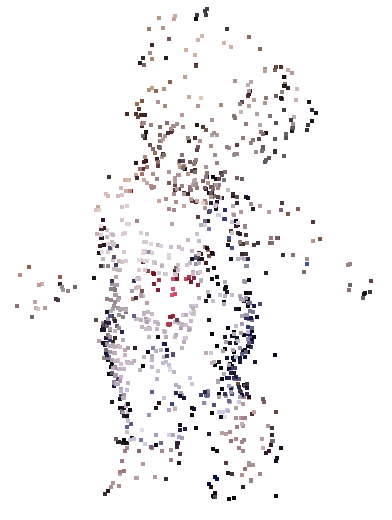
\includegraphics[width=0.3\textwidth]{img/bjorn}  %\label{fig:}
 }
  \caption{Reconstructed sparse point cloud of stuffed toy}
 \label{fig:bjorn}
\end{figure}
